\documentclass[12pt]{article}
\usepackage[paper=letterpaper, left=1in, right=1in, top=1in, bottom=1in]{geometry}

\usepackage[parfill]{parskip}
\usepackage{amssymb}
\usepackage{amsmath}
\usepackage{tikz}
\usetikzlibrary{patterns}

\begin{document}

\begin{center}
\Large{CS 191\\}
\large{Homework 2\\}
\end{center}
\begin{flushright}
Cameron Moberg\\
cjm8713\\
\today\\
\end{flushright}

\textbf{Problem 1.}  Show the power set of the set $\{q,r,s\}$.\\
\textit{Answer:} The power set is: \\ 
$\{\},\{q\},\{r\},\{s\},\{q,s\},\{r,s\},\{q,r\},\{q,r,s\}$

\vspace{7mm}
\textbf{Problem 2.}

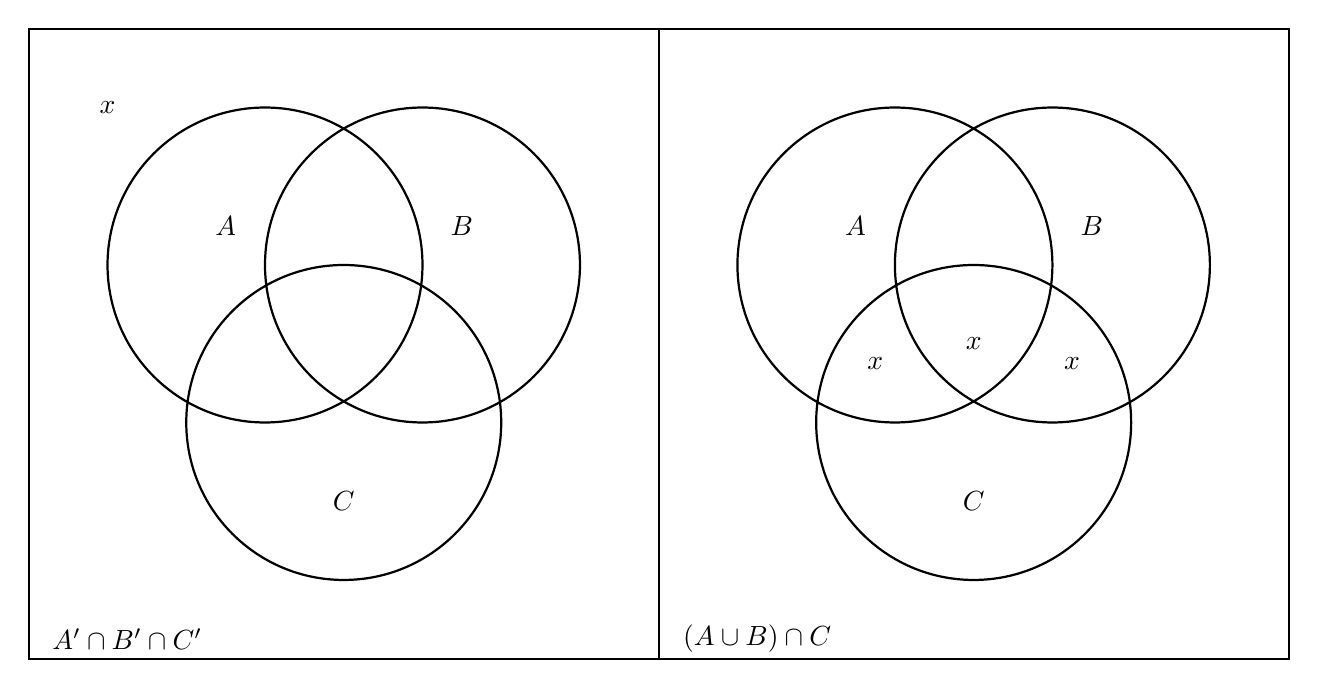
\begin{tikzpicture}[thick,fill opacity=1]
\draw (0,0) rectangle (16,8);
\draw (8,8) -- (8,0);
\draw (3,5) circle (2cm)   (5,5) circle (2cm)  (4,3) circle (2cm);
\draw (11,5) circle (2cm)   (13,5) circle (2cm)  (12,3) circle (2cm);

\draw(1.25,.25) node[opacity=1] {$A' \cap B' \cap C'$};
\draw(2.5,5.5) node {$A$};
\draw(5.5,5.5) node {$B$};
\draw(4,2) node {$C$};
\draw(1,7) node[opacity=1] {$x$};


\draw(9.25,.25) node[opacity=1] {$(A \cup B) \cap C$};
\draw(10.5,5.5) node {$A$};
\draw(13.5,5.5) node {$B$};
\draw(12,2) node {$C$};
\draw(12,4) node[opacity=1] {$x$};
\draw(10.75,3.75) node[opacity=1] {$x$};
\draw(13.25,3.75) node[opacity=1] {$x$};

\end{tikzpicture}


\textbf{Section 1.2}\\

\textbf{Exercise 8.a:} Let $A=\{6k+5 | k \in \mathbb{N}\}$ and $B=\{3k+2|k \in \mathbb{N}\}$, show that $A \subseteq B$.  \\ 
\textit {Answer:} To prove this we must assume that $x \in A$ so $x = 6k+5$ for some $k \in \mathbb{N}$. If $x=6k+5$ then $x=6k+3+2=3(2k+1)+2$, but $2k+1 \in \mathbb{N}$ or else the proof does not work. So $x \in B$ assuming that $x \in A$ meaning that $A \subseteq B$. \\

\textbf{Exercise 10:} Find the set $A$ that satisfies the following two properties: \\
$A \cap \{3,4,5,6\} = \{1,2,3,4,5,6\}\\
A \cup \{3,4,5,6\} = \{3,4\}$\\
\textit {Answer:} 
$A \cap \{3,4,5,6\} = \{1,2,3,4,5,6\} = \{1,2\} \\
A \cup \{3,4,5,6\} = \{3,4\} = \{3,4\}$\\
Therefore $A = \{1,2,3,4\}$\\

\textbf{Exercise 14.a:} Sets are indicated by the letter $x$ Find an expression for each of the three sets in terms of set operations.

\begin{tikzpicture}
\draw(0,0) rectangle (15,8);
\draw(7.5,0) -- (7.5,8);
\draw(7.5/2,0) rectangle (7.5+7.5/2,-8);

%top left
\draw (2.75,5) circle (2cm)   (4.75,5) circle (2cm)  (3.75,3) circle (2cm);
\draw(1.75,6) node {$A$};
\draw(5.75,6) node {$B$};
\draw(3.75,1.5) node {$C$};
\draw(.25,.25) node {$a.$};
\draw(3.75,6) node {$x$}; 
\draw(3.75,.3) node{$(A \cap B) -C$};
%top right
\draw (10.25,5) circle (2cm)   (12.25,5) circle (2cm)  (11.25,3) circle (2cm);
\draw(9.25,6) node {$A$};
\draw(13.25,6) node {$B$};
\draw(11.25,1.5) node {$C$};
\draw(7.75,.25) node {$b.$};
\draw(11.2 5,6) node {$x$}; 
\draw(12.75,5.5) node{$x$};
\draw(12.25,3.75) node{$x$};
\draw(11.25,2.5) node{$x$};
\draw(11.25,.3) node{$(B \cup C) - (C \cap A)$};
%bottom middle
\draw (6.5,-3) circle (2cm)   (8.5,-3) circle (2cm)  (7.5,-5) circle (2cm);
\draw(5.5,-2) node {$A$};
\draw(9.5,-2) node {$B$};
\draw(7.5,-6.5) node {$C$};
\draw(4,-7.75) node {$c.$};
\draw(7.5,-2) node {$x$};
\draw(9,-2.5) node {$x$};
\draw(7.5,-5.5) node {$x$};
\draw(6.5,-4.25) node{$x$};
\draw(7.5,-7.70) node{$B \oplus C$};
\end{tikzpicture}

\textit{Answer:}\\
$a.$ $ (A \cap B) -C$\\
$b.$ $ (B \cup C) - (C \cap A)$\\
$c.$ $ B \oplus C$
\end{document}
